\documentclass{article}

\usepackage[UTF8]{ctex}
\usepackage{amsmath,amssymb}
\usepackage{geometry}
\usepackage{graphicx}
\usepackage{float}

\geometry{a4paper, margin=2.5cm}

\begin{document}

% ============================================================
\section*{策略梯度（Policy Gradient / REINFORCE）}

\subsection*{先讲一个故事}

DQN 之后，我们已经能让 AI 在 Atari 游戏上打败人类。但有人提出了一个问题：DQN 的本质是「找到每个状态下最好的动作」——这套逻辑在动作是离散的时候很好用，但如果要控制一只机械手臂呢？

机械手臂的每个关节角度是连续值，动作空间无限大，根本列不出一张 Q 表，也没法对所有动作取最大值。而且更根本的问题是：DQN 学的是「哪个动作最好」（Q 函数），它绕了一圈，并没有直接告诉你「应该用什么策略」。

有没有一种更直接的方式——\textbf{直接优化策略本身}？

这就是 \textbf{策略梯度（Policy Gradient）}的出发点：不学 Q 值，改学一个参数化的策略 $\pi(a \mid s; \theta)$，通过梯度上升让它越来越好。REINFORCE 是这条路上最原始也最重要的算法。

\textbf{本章的核心问题}：怎么对一个策略求梯度？

% ============================================================
\section*{从 Q 值到策略}

\subsection*{两种 RL 的哲学}

\begin{itemize}
  \item \textbf{基于价值（Value-based）}：先学 $Q(s,a)$，再从 Q 值派生出策略（如 $\varepsilon$-贪心）。DQN 属于这一类。
  \item \textbf{基于策略（Policy-based）}：直接参数化策略 $\pi_\theta$，最大化期望总回报 $J(\theta) = \mathbb{E}_{\tau \sim \pi_\theta}[R(\tau)]$。
\end{itemize}

策略梯度的优势：
\begin{itemize}
  \item 天然支持连续动作（输出均值和方差，从高斯分布采样）；
  \item 策略是随机的（stochastic），内置探索，不需要额外的 $\varepsilon$-贪心；
  \item 优化目标平滑，收敛性有一定理论保证。
\end{itemize}

\subsection*{问题：$J(\theta)$ 对 $\theta$ 的梯度怎么算？}

期望总回报是一个轨迹上的期望，而轨迹的分布又依赖 $\theta$——对一个依赖参数的期望求梯度，不能直接交换梯度和期望符号。

% ============================================================
\section*{对数导数技巧（Log-Derivative Trick）}

关键恒等式：
\[
\nabla_\theta \pi_\theta(a \mid s) = \pi_\theta(a \mid s) \cdot \nabla_\theta \log \pi_\theta(a \mid s)
\]

利用这个技巧，可以把对分布的梯度转化为期望内部的梯度：
\[
\boxed{\nabla_\theta J(\theta) = \mathbb{E}_{\tau \sim \pi_\theta}\!\left[\sum_{t=0}^{T} \nabla_\theta \log \pi_\theta(a_t \mid s_t) \cdot G_t \right]}
\]

其中 $G_t = \sum_{k=t}^{T} \gamma^{k-t} r_k$ 是从第 $t$ 步开始的折扣回报。

\textbf{直觉}：这个梯度的含义很漂亮——$G_t$ 大（这条路走得好），就增大 $\log \pi(a_t \mid s_t)$（让这个动作更可能发生）；$G_t$ 小，就降低它的概率。\textbf{好的行为得到强化，坏的行为被压制}。

% ============================================================
\section*{REINFORCE 算法}

策略梯度定理告诉我们梯度的形式，但期望无法精确计算——用 Monte Carlo 采样估计它：

\begin{enumerate}
  \item 用当前策略 $\pi_\theta$ 完整地跑一个 episode，收集轨迹 $\{(s_t, a_t, r_t)\}$；
  \item 计算每步的折扣回报 $G_t$（从轨迹末尾反向累加）；
  \item 用梯度估计更新参数：
\end{enumerate}
\[
\boxed{\theta \leftarrow \theta + \alpha \sum_{t} \nabla_\theta \log \pi_\theta(a_t \mid s_t) \cdot G_t}
\]

这就是 \textbf{REINFORCE} 算法（Williams, 1992）。完整跑一个 episode 才做一次更新，用回报 $G_t$ 作为「信号强弱」来缩放梯度——简洁优雅，但有一个致命弱点。

% ============================================================
\section*{高方差：REINFORCE 的软肋}

Monte Carlo 估计有无偏性（无数次采样的均值等于真实期望），但方差极大：
\begin{itemize}
  \item 同一个状态 $s$，不同 episode 下的回报 $G_t$ 可能从 10 到 500 都有；
  \item 策略更新完全依赖单条轨迹的运气——运气好就大幅强化，运气差就大幅抑制；
  \item 学习曲线剧烈抖动，有时突然冲高，又迅速掉回来，难以稳定收敛。
\end{itemize}

实验如图~\ref{fig:variance} 所示：5 个随机种子的原始训练曲线波动巨大，平滑均值始终维持在低水平，vanilla REINFORCE 在 500 集内无法稳定解决 CartPole-v1。

\begin{figure}[H]
  \centering
  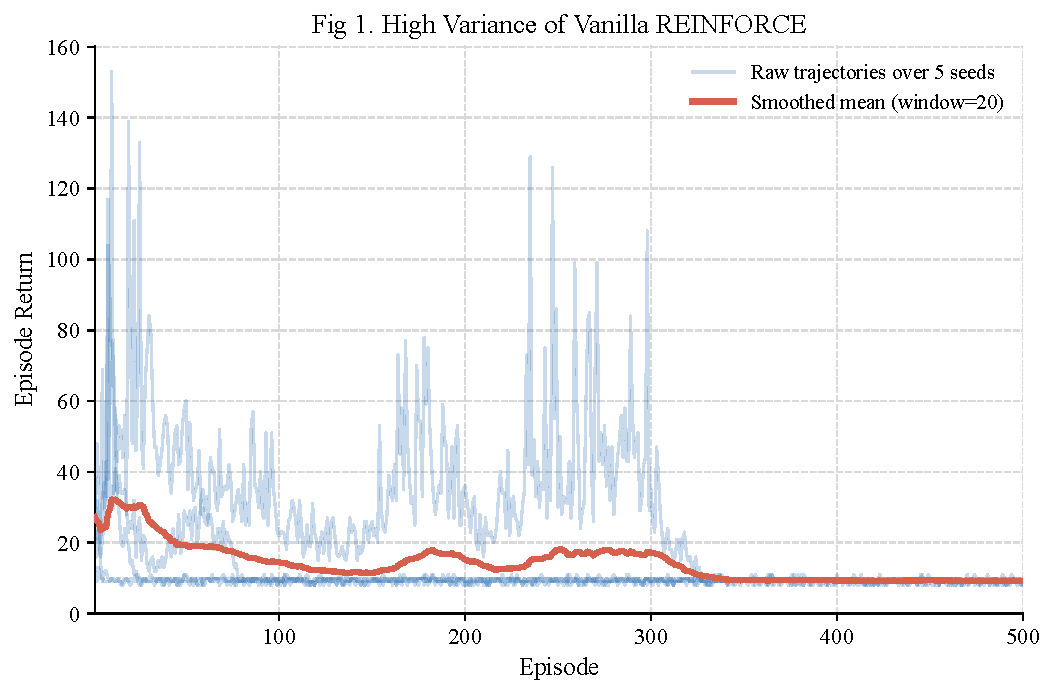
\includegraphics[width=0.95\textwidth]{fig1_reinforce_high_variance.pdf}
  \caption{Vanilla REINFORCE 的高方差（CartPole-v1，5 个随机种子）。原始轨迹剧烈波动，部分 episode 短暂冲高但随即回落，平滑均值长期维持在较低水平。}
  \label{fig:variance}
\end{figure}

% ============================================================
\section*{方差缩减：Value Baseline}

\subsection*{核心思路}

方差大的根源：$G_t$ 这个数字本身就很大（CartPole 满分 500），用它直接缩放梯度，导致更新步长飘忽不定。

解决思路：不用 $G_t$，改用「这次比平均水平好多少」——即\textbf{优势函数（Advantage）}：
\[
\boxed{A_t = G_t - V(s_t)}
\]

其中 $V(s_t)$ 是对当前状态期望回报的估计（Baseline）。减去均值后，$A_t$ 在 0 附近波动，方差大幅降低。

\subsection*{为什么减去 Baseline 不影响梯度方向？}

可以证明，任何只依赖状态（不依赖动作）的函数 $b(s)$ 满足：
\[
\mathbb{E}_{\tau \sim \pi_\theta}\!\left[\nabla_\theta \log \pi_\theta(a_t \mid s_t) \cdot b(s_t)\right] = 0
\]

因此减去 $V(s_t)$ 不改变梯度的\textbf{期望}，只降低\textbf{方差}——是一个方差缩减（variance reduction）技巧，在统计学中称为控制变量法。

\subsection*{实践：用神经网络估计 $V(s)$}

在实际的 REINFORCE with Baseline 中：
\begin{itemize}
  \item 额外维护一个 \textbf{Value Network} $V(s;\phi)$，通过最小化均方误差 $\mathcal{L}(\phi) = \mathbb{E}[(G_t - V(s_t;\phi))^2]$ 来训练；
  \item Policy 梯度改为 $\nabla_\theta \log \pi_\theta(a_t \mid s_t) \cdot A_t$；
  \item $V(s)$ 的学习率须\textbf{低于} policy 的学习率——若 $V(s)$ 收敛太快（几乎完美拟合 $G_t$），则 $A_t \approx 0$，policy 的梯度信号消失。
\end{itemize}

消融实验如图~\ref{fig:baseline} 所示。

\begin{figure}[H]
  \centering
  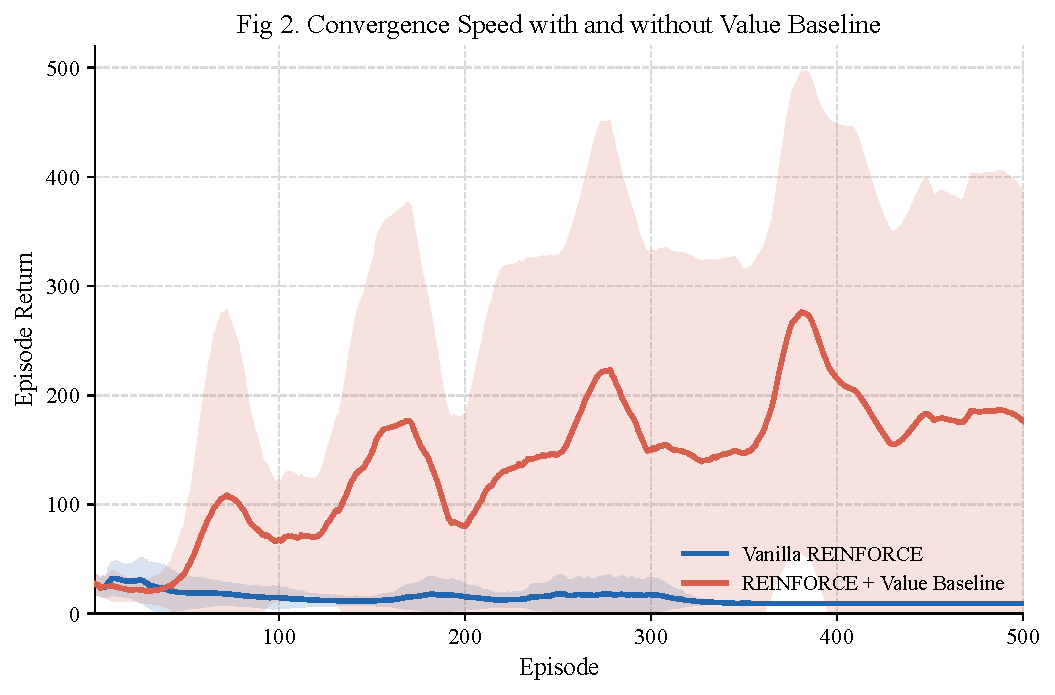
\includegraphics[width=0.88\textwidth]{fig2_convergence_baseline_comparison.pdf}
  \caption{有 / 无 Value Baseline 的训练对比（CartPole-v1，5 个随机种子，阴影为 $\pm 1\sigma$）。加入 Baseline 后，部分种子能在 500 集内收敛到接近满分，整体期望回报显著高于 Vanilla REINFORCE。}
  \label{fig:baseline}
\end{figure}

% ============================================================
\section*{策略熵：从随机到确定}

\textbf{策略熵}定义为：
\[
H(\pi(\cdot \mid s)) = -\sum_a \pi(a \mid s) \log \pi(a \mid s)
\]

对于 CartPole 的二动作环境，均匀随机策略的熵最大为 $\ln 2 \approx 0.693$ nats。熵下降，意味着策略从「乱按按键」走向「确定选择」。

图~\ref{fig:entropy} 展示了两种方法在训练过程中的熵演化：

\begin{figure}[H]
  \centering
  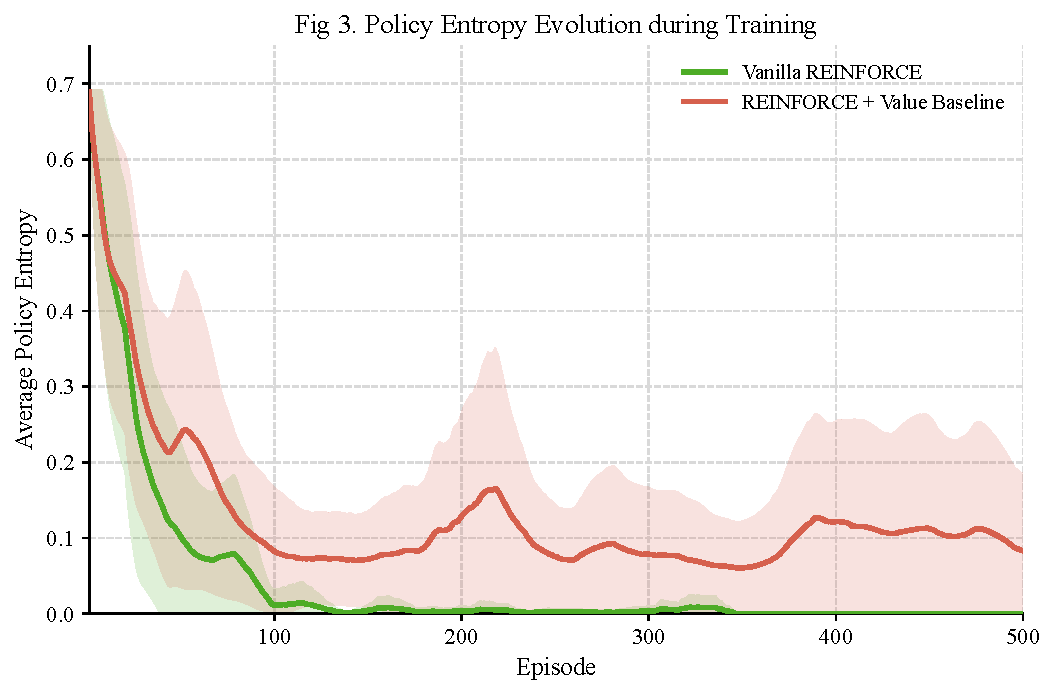
\includegraphics[width=0.88\textwidth]{fig3_policy_entropy_evolution.pdf}
  \caption{策略熵在训练过程中的演化（CartPole-v1，5 个随机种子，阴影为 $\pm 1\sigma$）。Vanilla REINFORCE 熵迅速塌缩至接近 0，但并未收敛到好策略，是过早陷入坏的确定性策略；有 Baseline 的版本熵下降更平缓，保留探索能力，最终收敛到更好的策略。}
  \label{fig:entropy}
\end{figure}

两条曲线对比揭示了一个有趣的现象：熵快速下降并不代表「学得好」——Vanilla REINFORCE 的熵在约 100 集后几乎归零，但对应的 return 仍然很低（图~\ref{fig:variance}）。策略过早收敛到一个糟糕的确定性行为（比如始终向一个方向推），探索能力丧失，无法继续改进。Value Baseline 通过提供更稳定的学习信号，让策略得以持续探索，才有机会发现更优的行为模式。

% ============================================================
\section*{完整算法：REINFORCE with Value Baseline}

\begin{enumerate}
  \item \textbf{初始化}：Policy Network $\pi(a \mid s;\theta)$，Value Network $V(s;\phi)$；
  \item \textbf{每个 episode}：
    \begin{enumerate}
      \item 用 $\pi_\theta$ 跑完整一集，收集 $\{(s_t, a_t, r_t)\}_{t=0}^T$；
      \item 反向计算折扣回报：$G_t = \sum_{k=t}^T \gamma^{k-t} r_k$；
      \item 更新 Value Network：$\phi \leftarrow \phi - \alpha_V \nabla_\phi \sum_t (G_t - V(s_t;\phi))^2$；
      \item 计算优势：$A_t = G_t - V(s_t;\phi)$（detach，不回传梯度）；
      \item 更新 Policy Network：$\theta \leftarrow \theta + \alpha_\pi \sum_t \nabla_\theta \log \pi_\theta(a_t \mid s_t) \cdot A_t$。
    \end{enumerate}
\end{enumerate}

\textbf{关键超参数注意事项}：

\[
\begin{array}{l|l}
\textbf{设置} & \textbf{原因} \\
\hline
\alpha_V < \alpha_\pi & V(s) 不能过快收敛，否则 A_t \approx 0，梯度信号消失 \\[4pt]
\text{不对 } A_t \text{ 做 z-score} & V(s) 已提供自然的中心化，再归一化易消灭信号 \\[4pt]
\text{clip\_grad\_norm} & 单条轨迹梯度方差大，梯度裁剪防止步长过大 \\
\end{array}
\]

% ============================================================
\section*{Policy Gradient 在 RL 体系中的位置}

REINFORCE 是策略梯度方法的起点，承接经典 RL，开启 Actor-Critic 主线：

\begin{enumerate}
  \item \textbf{从价值到策略}：Q-learning / DQN 优化 $Q$ 函数，间接得到策略；Policy Gradient 直接优化 $\pi_\theta$，目标更清晰，天然支持连续动作空间；
  \item \textbf{Monte Carlo 的代价}：REINFORCE 等整集结束才更新，数据效率低，方差大；这催生了下一步的改进；
  \item \textbf{Actor-Critic（A2C/A3C）}：把 REINFORCE 中的 Monte Carlo 回报 $G_t$ 换成 TD 估计（Bootstrapping），不等 episode 结束就更新。Actor（Policy）和 Critic（Value）协同训练，方差和偏差均衡；
  \item \textbf{PPO / TRPO}：在 Actor-Critic 基础上加入策略更新幅度约束，防止一步更新破坏策略；PPO 是目前工业界最广泛使用的策略梯度算法，ChatGPT 的 RLHF 训练正是基于它；
  \item \textbf{连续控制主线}：DDPG、TD3、SAC 把策略梯度扩展到连续动作空间，成为机器人控制的主流方法。
\end{enumerate}

\subsection*{参考资料}

\begin{enumerate}
  \item Williams, R.\,J.\ (1992). Simple statistical gradient-following algorithms for connectionist reinforcement learning. \textit{Machine Learning}, 8, 229--256.
  \item Sutton, R.\,S.\ \& Barto, A.\,G.\ (2018). \textit{Reinforcement Learning: An Introduction} (2nd ed.). Chapter 13: Policy Gradient Methods.
  \item Schulman, J., et al.\ (2015). Trust Region Policy Optimization. \textit{ICML}.
  \item Schulman, J., et al.\ (2017). Proximal Policy Optimization Algorithms. \textit{arXiv:1707.06347}.
  \item 动手学强化学习（Hands-on-RL）. 第 9 章：策略梯度算法.
\end{enumerate}

\end{document}
